\chapter{Heterogeneity}
\label{chap:five}
% grammar checked (07-26)

Thus far, my analysis has focused primarily on the relationship between the true effect and its standard error. Several methods from the previous chapter, such as the \ac{IV} regression, p-uniform*, or \ac{RoBMA}, provided us with a quick glimpse into the topic of systematic heterogeneity. However, none delivered a more complex overview of the data's nature. This chapter aims to do precisely that - delve deeper into the study design and search for systematic patterns that may reveal more about the behavior of the effect. For this purpose, I will utilize two methods, \ac{BMA} and \ac{FMA}. These should help me identify the influence of different variables on the effect behavior and quantitatively capture the magnitude of this influence. Before constructing any models, however, it is crucial to explain and explore the dataset structure first.

\section{Variables}
\label{sec:variables}

I constructed the dataset aiming to comprehensively capture the most important categories that define the context of the collected data and the studies they come from. As such, I identified six categories, which I named as follows: the actual estimates along with their descriptive statistics, estimate characteristics, data characteristics, spatial/structural variation, estimation method, and publication characteristics. Across these six categories, I collected 37 distinct variable groups. Note that a group here could mean either a standalone variable (i.e., data year) or a group of variables (i.e., low/middle/high-income country). In the latter case, the variable groups consist either of dummies, or ratios, such as the ratio of subjects living in an urban area. The list of all quantifiable, relevant variables can be found in \autoref{tab:var}. To keep visual clarity, I excluded variables that could not be easily quantified, such as the country where the study was conducted, or variables irrelevant to the effect behavior explanation, such as observation id.

%BMA+FMA variable description table
\begin{singlespace}
  \begin{scriptsize}
  \begin{longtable}{
  @{\hskip\tabcolsep\extracolsep\fill}
  l
  %p{0.25\hsize}
  p{0.55\hsize}
  cc
  @{}
  } %0.15 0.65
  \caption{Definition and summary statistics of regression variables}  \label{tab:var}\\
  \toprule
    \multicolumn{1}{l}{Variable} &   \multicolumn{1}{l}{Description} &         \multicolumn{1}{c}{Mean} &           \multicolumn{1}{c}{SD} \\
  \midrule
  \endfirsthead
  \caption[]{Definition and summary statistics of regression variables (continued)}\\
  \toprule
    \multicolumn{1}{l}{Variable} &   \multicolumn{1}{l}{Description} &         \multicolumn{1}{c}{Mean} &           \multicolumn{1}{c}{SD} \\
  \midrule
  \endhead
  \bottomrule
  \multicolumn{4}{r}{{\scriptsize Continued on next page}} \\
  \endfoot
  \endlastfoot
  Effect & The effect of an additional year of schooling on logarithmic wage. & 7.476 & 4.439 \\
  Standard Error & The standard error of the main effect. & 1.284 & 1.693 \\
  \midrule
  
  \multicolumn{4}{l}{\emph{Estimate characteristics}}\\
  Estimate: City & =1 if the estimates within the study can be aggregated on a city level. & 0.119 & 0.323 \\
  Estimate: Sub-region & =1 if the estimates within the study can be aggregated on a subregional level. & 0.099 & 0.299 \\
  Estimate: Region & =1 if the estimates within the study can be aggregated on a regional level. & 0.309 & 0.462 \\
  Estimate: Country & =1 if the estimates within the study can be aggregated on a country level. & 0.395 & 0.489 \\
  Estimate: Continent & =1 if the estimates within the study can not be aggregated on a country level or smaller (reference category). & 0.079 & 0.269 \\
  \midrule
  
  \multicolumn{4}{l}{\emph{Data characteristics}}\\
  Study Size & The logarithm of the number of estimates collected from the study. & 2.942 & 0.637 \\
  Yrs. of Schooling & The average number of years of schooling attained by the subjects. & 11.116 & 3.461 \\
  Yrs. of Experience & The average number of years of experience attained by the subjects. & 18.351 & 7.450 \\
  Education: Years & =1 if authors report schooling in years. & 0.634 & 0.482 \\
  Education: Levels & =1 if the authors report schooling in levels (e.g., attained college degree) (reference category). & 0.366 & 0.482 \\
  Wage: Log Hourly & =1 if the dependent variable in the regression is log hourly wage. & 0.531 & 0.499 \\
  Wage: Log Daily & =1 if the dependent variable in the regression is log daily or weekly wage. & 0.095 & 0.293 \\
  Wage: Log Monthly & =1 if the dependent variable in the regression is log monthly wage. & 0.211 & 0.408 \\
  Wage: Annual Earnings & =1 if the dependent variable in the regression is log of mean annual earnings (reference category). & 0.162 & 0.369 \\
  Micro Data & =1 if the study uses micro data. & 0.177 & 0.382 \\
  Survey Data & =1 if the study uses data from a survey. & 0.534 & 0.499 \\
  National Register Data & =1 if the study uses data from a national register (reference category). & 0.289 & 0.453 \\
  Cross-sectional Data & =1 if the study uses cross-sectional data. & 0.361 & 0.481 \\
  Panel Data & =1 if the study uses panel data (reference category). & 0.639 & 0.481 \\
  Data Year & The logarithm of the average year of the study's time span & 7.599 & 0.006 \\
  \midrule
  
  \multicolumn{4}{l}{\emph{Spatial/structural variation}}\\
  No Education & The percentage of subjects that attained no education (reference category). & 0.126 & 0.148 \\
  Primary Education & The percentage of subjects that attained only primary education. & 0.177 & 0.151 \\
  Secondary Education & The percentage of subjects that attained only secondary education. & 0.388 & 0.196 \\
  Higher Education & The percentage of subjects that attained any form of higher education. & 0.309 & 0.247 \\
  Wage Earners & The ratio of wage earners to self-employed subjects in the study ( = 1 if wage earner, = 0 if self-employed). & 0.837 & 0.205 \\
  Self-Employed & The ratio of self-employed to wage earners subjects in the study ( = 1 if self-employed, = 0 if wage earner) (reference category). & 0.163 & 0.205 \\
  Male & The ratio of male to female subjects in the study ( = 1 if male, = 0 if female). & 0.650 & 0.350 \\
  Female & The ratio of female to male subjects in the study ( = 1 if female, = 0 if male) (reference category). & 0.350 & 0.350 \\
  Private Sector & The ratio of private to public sector workers ( = 1 if private sector worker, = 0 if public). & 0.596 & 0.163 \\
  Public Sector & The ratio of public to private sector workers ( = 1 if public sector worker, = 0 if private) (reference category). & 0.404 & 0.163 \\
  Ethnicity: Caucasian & The ratio of Caucasian to non-Caucasian subjects in the study ( = 1 if Caucasian, = 0 if not). & 0.227 & 0.419 \\
  Ethnicity: Other & The ratio of non-Caucasian to Caucasian subjects in the study ( = 1 if non-Caucasian, = 0 if Caucasian) (reference category). & 0.773 & 0.419 \\
  Rural & The ratio of rural to urban workers ( = 1 if rural worker, = 0 if urban). & 0.297 & 0.191 \\
  Urban & The ratio of urban to rural workers ( = 1 if urban worker, = 0 if rural) (reference category). & 0.703 & 0.191 \\
  Reg: Advanced Econ. & =1 if the study was conducted in a country with advanced economy. (reference group) & 0.498 & 0.500 \\
  High Income Countries & =1 if the study was conducted in a high income country (reference category) & 0.507 & 0.500 \\
  Median Expenditure & The logarithm of the median expenditure in the country in a given year. & 8.584 & 1.420 \\
  Minimum Wage & The logarithm of the minimum wage in the country in a given year. & 5.853 & 1.536 \\
  Academic Freedom Index & The academic freedom index reported for the country in a given year. & 0.712 & 0.266 \\
  \midrule
  
  \multicolumn{4}{l}{\emph{Estimation method}}\\
  Method: OLS & =1 if the authors use Ordinary least squares (reference category). & 0.664 & 0.473 \\
  Method: Cohort/FE & =1 if the authors use Cohort-type or Fixed-effects estimation. & 0.058 & 0.234 \\
  Method: 2SLS & =1 if the authors use Two-Stage least squares estimation. & 0.095 & 0.294 \\
  Method: Heckman & =1 if the authors use Two-step estimation (Heckman and Polachek, 1974). & 0.062 & 0.240 \\
  Method: Probit & =1 if the authors use Probit estimation. & 0.022 & 0.147 \\
  Method: IV & =1 if the authors use Instrumental variables estimation. & 0.111 & 0.314 \\
  Ability: Direct & =1 if the authors include a direct measure of ability in their study. & 0.135 & 0.341 \\
  Ability: Proxied & =1 if the authors use a proxy for ability in their study. & 0.204 & 0.403 \\
  Ability: Uncontrolled & =1 if the authors acknowledge, but do not control for ability in any way in their study. & 0.425 & 0.494 \\
  Ability: Unmentioned & =1 if the authors do not mention ability anywhere in their study (reference category). & 0.223 & 0.417 \\
  Control: Age & =1 if the authors control for age in the regression. & 0.344 & 0.475 \\
  Control: Age$^2$ & =1 if the authors control for age in quadratic form in the regression. & 0.275 & 0.447 \\
  Control: Experience & =1 if the authors control for experience in the regression. & 0.607 & 0.489 \\
  Control: Experience$^2$ & =1 if the authors control for experience in quadratic form in the regression. & 0.512 & 0.500 \\
  Control: Ethnicity & =1 if the authors control for ethnicity in the regression. & 0.251 & 0.434 \\
  Control: Health & =1 if the authors control for health in the regression. & 0.135 & 0.342 \\
  Control: Gender & =1 if the authors control for gender in the regression. & 0.367 & 0.482 \\
  Control: Marriage & =1 if the authors control for marriage in the regression. & 0.361 & 0.480 \\
  Control: Occupation & =1 if the authors control for occupation of the subjects in the regression. & 0.142 & 0.349 \\
  Control: Firm Char. & =1 if the authors control for firm characteristics in the regression. & 0.149 & 0.357 \\
  Control: Area & =1 if the authors control for area type in the regression (e.g., urban, rural). & 0.418 & 0.493 \\
  Control: Macro Var. & =1 if the authors control for macroeconomic variables in the regression. & 0.347 & 0.476 \\
  \midrule
  
  \multicolumn{4}{l}{\emph{Publication characteristics}}\\
  Impact Factor & The logarithm of the Journal Citations Report impact factor of the study (as of January 2023; = 0 in case of no publication). & -0.906 & 1.533 \\
  Citations & The logarithm of the mean number of Google Scholar citations received per year since the appearance of the study in Google Scholar (as of January 2023). & 4.029 & 2.177 \\
  Study: Published & =1 if the study was published in a journal. & 0.764 & 0.425 \\
  Study: Unpublished & =1 if the study was not published in a journal (reference category). & 0.236 & 0.425 \\
  Publication Year & The logarithm of the number of years between the publication (or issuing) of this study and the publication year of the earliest published study in the sample. & 3.332 & 0.339 \\
  \bottomrule
     
   \multicolumn{4}{>{\scriptsize}p{0.95\linewidth}}{\emph{Note:} This table presents the summary statistics and descriptions for various study characteristics eligible for inclusion in Bayesian Model Averaging. Variables marked as \textit{reference categories} were automatically excluded from the procedure, as this would create a dummy variable trap. SD = standard deviation, OLS = Ordinary Least Squares, FE = Fixed Effects, 2SLS = 2 Stage Least Squares, IV = Instrumental Variable.}
  \end{longtable}
  \end{scriptsize}
  \end{singlespace}
  

Let us take a closer look at five of the six\footnote{The statistical properties of the estimate have already been described in \autoref{chap:three}.} variable categories and try to understand the reasoning behind my choices of this particular variable setup.

\subsection{Estimate Characteristics}
\label{subsec:estimate_char}

There are only a handful of variables that I identified as vital as far as effect characteristics are concerned. Moreover, variables such as the number of observations, or degrees of freedom, are not telling enough to be included in the model averaging. As such, the only full-fledged variable group included in this category is the estimate type, when divided into the size of the region. The estimates of over 70\% of studies in the dataset can be clustered into regional or country levels. Examples of such studies include \cite{walker2008college, fang2012returns}, or \cite{angrist1991compulsory}. Sporadically \citep{krafft2019what, chanis2021tell}, the authors focus on the city/sub-region level estimates or aggregate their results at a level of a continent or a group of countries.

\subsection{Data Characteristics}
\label{subsec:data_char}

Two variables are perhaps the most important in the category of data characteristics - \textit{years of schooling} and \textit{years of experience}. These represent the founding blocks of the Mincer equation and can be linked together using the age of subjects as described in \autoref{eq:potential_exp}. Across all studies in the data, the average reported number of schooling years equals 11.1, while 18.3 represents the average reported experience of subjects. Given that 781 observations in the data (roughly 44\% of all observations) are not directly reported, the \textit{years of experience} variable may be inflated by the calculation. Indeed, upon removing all observations that had to be manually calculated using \autoref{eq:potential_exp}, the average years of experience in the sample drops to 15.6. Nonetheless, to the best of my knowledge, there is no other way to circumvent this shortcoming. Consequently, I use the reported number of 18.3 in further calculations. To see examples of studies that fail to report years of schooling and/or experience, see \cite{pischke2005zero, psacharopoulos1982earnings}, while for studies that report both, see \cite{belzil2002unobserved, girma2005heterogeneity}.

Another crucial variable captures how education is reported - years or levels\footnote{See \autoref{sec:effect_meaning} for more details about this classification.} In about two-thirds of all studies, years of attained education is used instead of the highest attained level (primary school, secondary school, etc.). It should be noted here that in cases a study reported both types, but the results captured the same outcome, I chose to collect only the number of years and discard the estimates in levels. This is to avoid collecting duplicate results. \cite{harmon2002returns} is an excellent example of a study that utilizes reporting of schooling years, while \cite{duraisamy2002changes} provides a counterexample.

The last variable worth a mention from this category is the variable denoting cross-section/panel data. Initially, I coded a short/long run variable under the \textit{estimate characteristics} that divided studies according to their run-time into those of length above and below one year. However, after the collection, I found that the cross-section/panel variable almost entirely captured this information, so I kept only this variable in the data. Nearly two-thirds of the collected experiments work with panel data such as longitudinal surveys (see \cite{harmon2003returns}). On the other hand, one-third of them deal with cross-sectional data (\cite{lemieux2001education} as an example).

The rest of the variables in this category is self-explanatory. For the complete list, see \autoref{tab:var}.

\subsection{Spatial/Structural Variation}
\label{subsec:spat_str_variation}

A whole array of variables that capture study variation are all coded under the category \textit{spatial/structural variation}. In most cases, this refers to either characteristics of the study subjects or the country in which the study is conducted. Pointing out a handful of crucial statistics that tie to these variables, we can see that most of the data sample consists of wage workers (83.7\%), 65\% of the subjects are male, 22.7\% come from the Caucasian ethnicity, 70.3\% live in the urban area, about half of them (49.8\%) come from a country with an advanced economy, and their average age is 35.69. To see the rest of the statistics, see \autoref{tab:var}.

% Here perhaps mention that age had to be dropped from the BMA to avoid the dummy trap

Most of the choices regarding the variables themselves should be more or less straightforward. As such, I would like to focus on the calculation behind some of these instead. For example, the variables \textit{median expenditure} and \textit{minimum wage} are notably coded on the country-year level, meaning a data point exists for every unique country-year pair. This is to account for country-level heterogeneity, as well as inflation. Another variable, the \textit{academic freedom index}, is too coded in this way.

Some variables, such as the rural/urban sector, are set up as ratios. For example, \cite{paweenawat2015private}, report exactly 47.4\% of subjects that live in rural areas, and 57.6\% that live in urban ones. This variable structure allows us to retain more information while behaving as a simple dummy in case only one of the alternatives is present in the data, such as when all subjects live in a city. I also employ this ratio-type setup with multiple categories in the variable that denotes the highest attained education. Here, the choices are split between primary, secondary, and higher education, as well as no education. When the authors report only several of these but not all, such as in the case of \cite{chanis2021tell}, I set the remaining variable categories to 0.

A more complex issue arises when more data points are missing, however. As an example, 32.5\% of the 1754 studies do not report whether their subject pool consists of wage workers or self-employed individuals. 53.4\% then omit the information on area type (urban/rural), and 60.5\% fail to specify whether the subjects work in a private or a public sector. To run the model averaging, the dataset has to contain no missing points in the employed variables. As such, I resort to interpolation, whose specifics I explained earlier in \autoref{chap:three}.

\subsection{Estimation Method}
\label{subsec:estim_method}

Regarding the actual estimation of the Mincer equation, the practices literature can be explained by three major variable sub-categories. Firstly, the estimation method used by the studies. Two-thirds of studies in the dataset (66.4\%) use simple \ac{OLS} for the estimation, while the rest use one of several other methods, including the Fixed-effects, Probit model, Instrumental variable regression, or Two-stage least squares. Several studies, such as \cite{debrauw2008reconciling}, employ a two-step estimation described in \cite{heckman1974empirical}.

Secondly, the \textit{ability} variable, described in \autoref{chap:two}, is also coded here. We can see that 13.5\% of studies include ability directly in the regression, 20.4\% use a proxy of some kind, 42.5\% do not control for ability but are aware of it, and 22.3\% do not mention ability or ability bias in any way.

Lastly, I add information on whether a study controls for variables such as age, experience, ethnicity, health, gender, marital status, etc. Usually, such as in the case of \cite{girma2005heterogeneity} or \cite{harmon2002returns}, only one of the two variables of age and experience are included. On the other hand, the included variable comes very frequently with the squared term, as described in the original Mincer equation. As for the other controls, there seems to be no obvious pattern in the studies, and the authors appear to be choosing the controls arbitrarily based on their study goals, data availability, or personal preferences.

\subsection{Publication Characteristics}
\label{subsec:pub_characteristics}

The last of the variable categories that I chose to employ denotes various publication characteristics of the included studies. The number of Google Scholar citations, the year of publication, or the Journal Citations Report impact factor are among the handful of variables within this category. As described in \autoref{chap:three}, I collected all journal/study data at a single time point, namely in January 2023. Although it is possible that the status of several of the included studies changed from then, I still value direct comparability more than keeping the information up-to-date with the latest changes.

Interestingly, but perhaps not surprisingly, 76.4\% of studies within the sample were published in a journal, and the mean number of citations for a study comes up to 56.2. This relatively high figure ties directly to the fact that roughly a third of the dataset consists of studies identified by snowballing - an activity aimed at targeting the most relevant and well-established relevant papers on the topic. Understandably, all of these papers have attained publication status, or their credibility would not be established.

With the variable setup out of the way, we can move on and employ these variables in exploring the effect behavior in a more detailed way.

\section{Model Averaging}
\label{sec:bma}

With the large number of variables my dataset holds, it is a rather complex and no doubt challenging task to pick those that could explain the effect behavior the best. Indeed, traditional methods such as \ac{OLS} are prone to over-specification bias, so simply dumping all collected variables into a single model does not appear like the best approach. Is there a way, then, where we could somehow discern the importance of the collected variables without knowing anything about them a priori? One such technique, called \ac{BMA}, appears suitable for the task and is precisely what the following sections will focus on.

Pioneered over two decades ago in papers such as \cite{hoeting1999bayesian} or \cite{raftery1997bayesian}, the technique provides a balanced approach that considers a multitude of statistically plausible models and assigns different weights to them using the Bayes' theorem and posterior inclusion probabilities. As explained in \cite{hoeting1999bayesian} and \cite{amini2011bayesian}, the process then highlights the importance of each variable based on these weights. For the procedures employed in this thesis, it is crucial to understand two metrics - \ac{PMP} and \ac{PIP}. For each variable, \ac{PMP} denotes how well each model fits the data. In contrast, \ac{PIP} is the sum of posterior model probabilities across the models in which that variable is included. The higher \ac{PIP}, the higher the variable's importance for explaining the effect's behavior.

I use a combination of the default Zellner's g-prior and the dilution prior for this particular analysis. The choice of the former stems from the fact that this setup allows for more control over collinearity in the data, an issue that may arise with the high number of variables. In my case, the number of eligible individual variables fed into the process once is 52 once reference variables are removed, making the collinearity treatment seem wise. \footnote{Here, an individual variable refers to each sub-group of a dummy variable group or any other variable that contains multiple categories. For example, the highest achieved education variable, as explained in \autoref{subsec:spat_str_variation}, would account for four individual variables (none, primary, secondary, and higher).}

Crucially, there exists one relationship among these variables that needs to be explicitly addressed at this point. Assuming that the equation \ref{eq:potential_exp} holds, the inclusion of all three variables of that relationship (years of schooling, years of experience, and age) in the model averaging would create a dummy variable trap. Removing one of these variables from the model averaging should solve this issue; I arbitrarily opt for subject age. As such, 51 variables are now marked as eligible for inclusion.

To ensure the carried information is unique for every variable, I also check the variance inflation factors of the included variables. This check revealed the sound design of the dataset, as all 51 variables, when lumped into a single model, hold a variance inflation factor no larger than 10. As for other parts of the setup, the last point of interest lies perhaps in the choice of the sampler, where I choose to use the default Markov Chain Monte Carlo algorithm \citep{zeugner2015bayesian}.

\begin{figure}[!htbp]
\begin{center}
\caption{Bayesian model averaging results}
\label{fig:BMA}
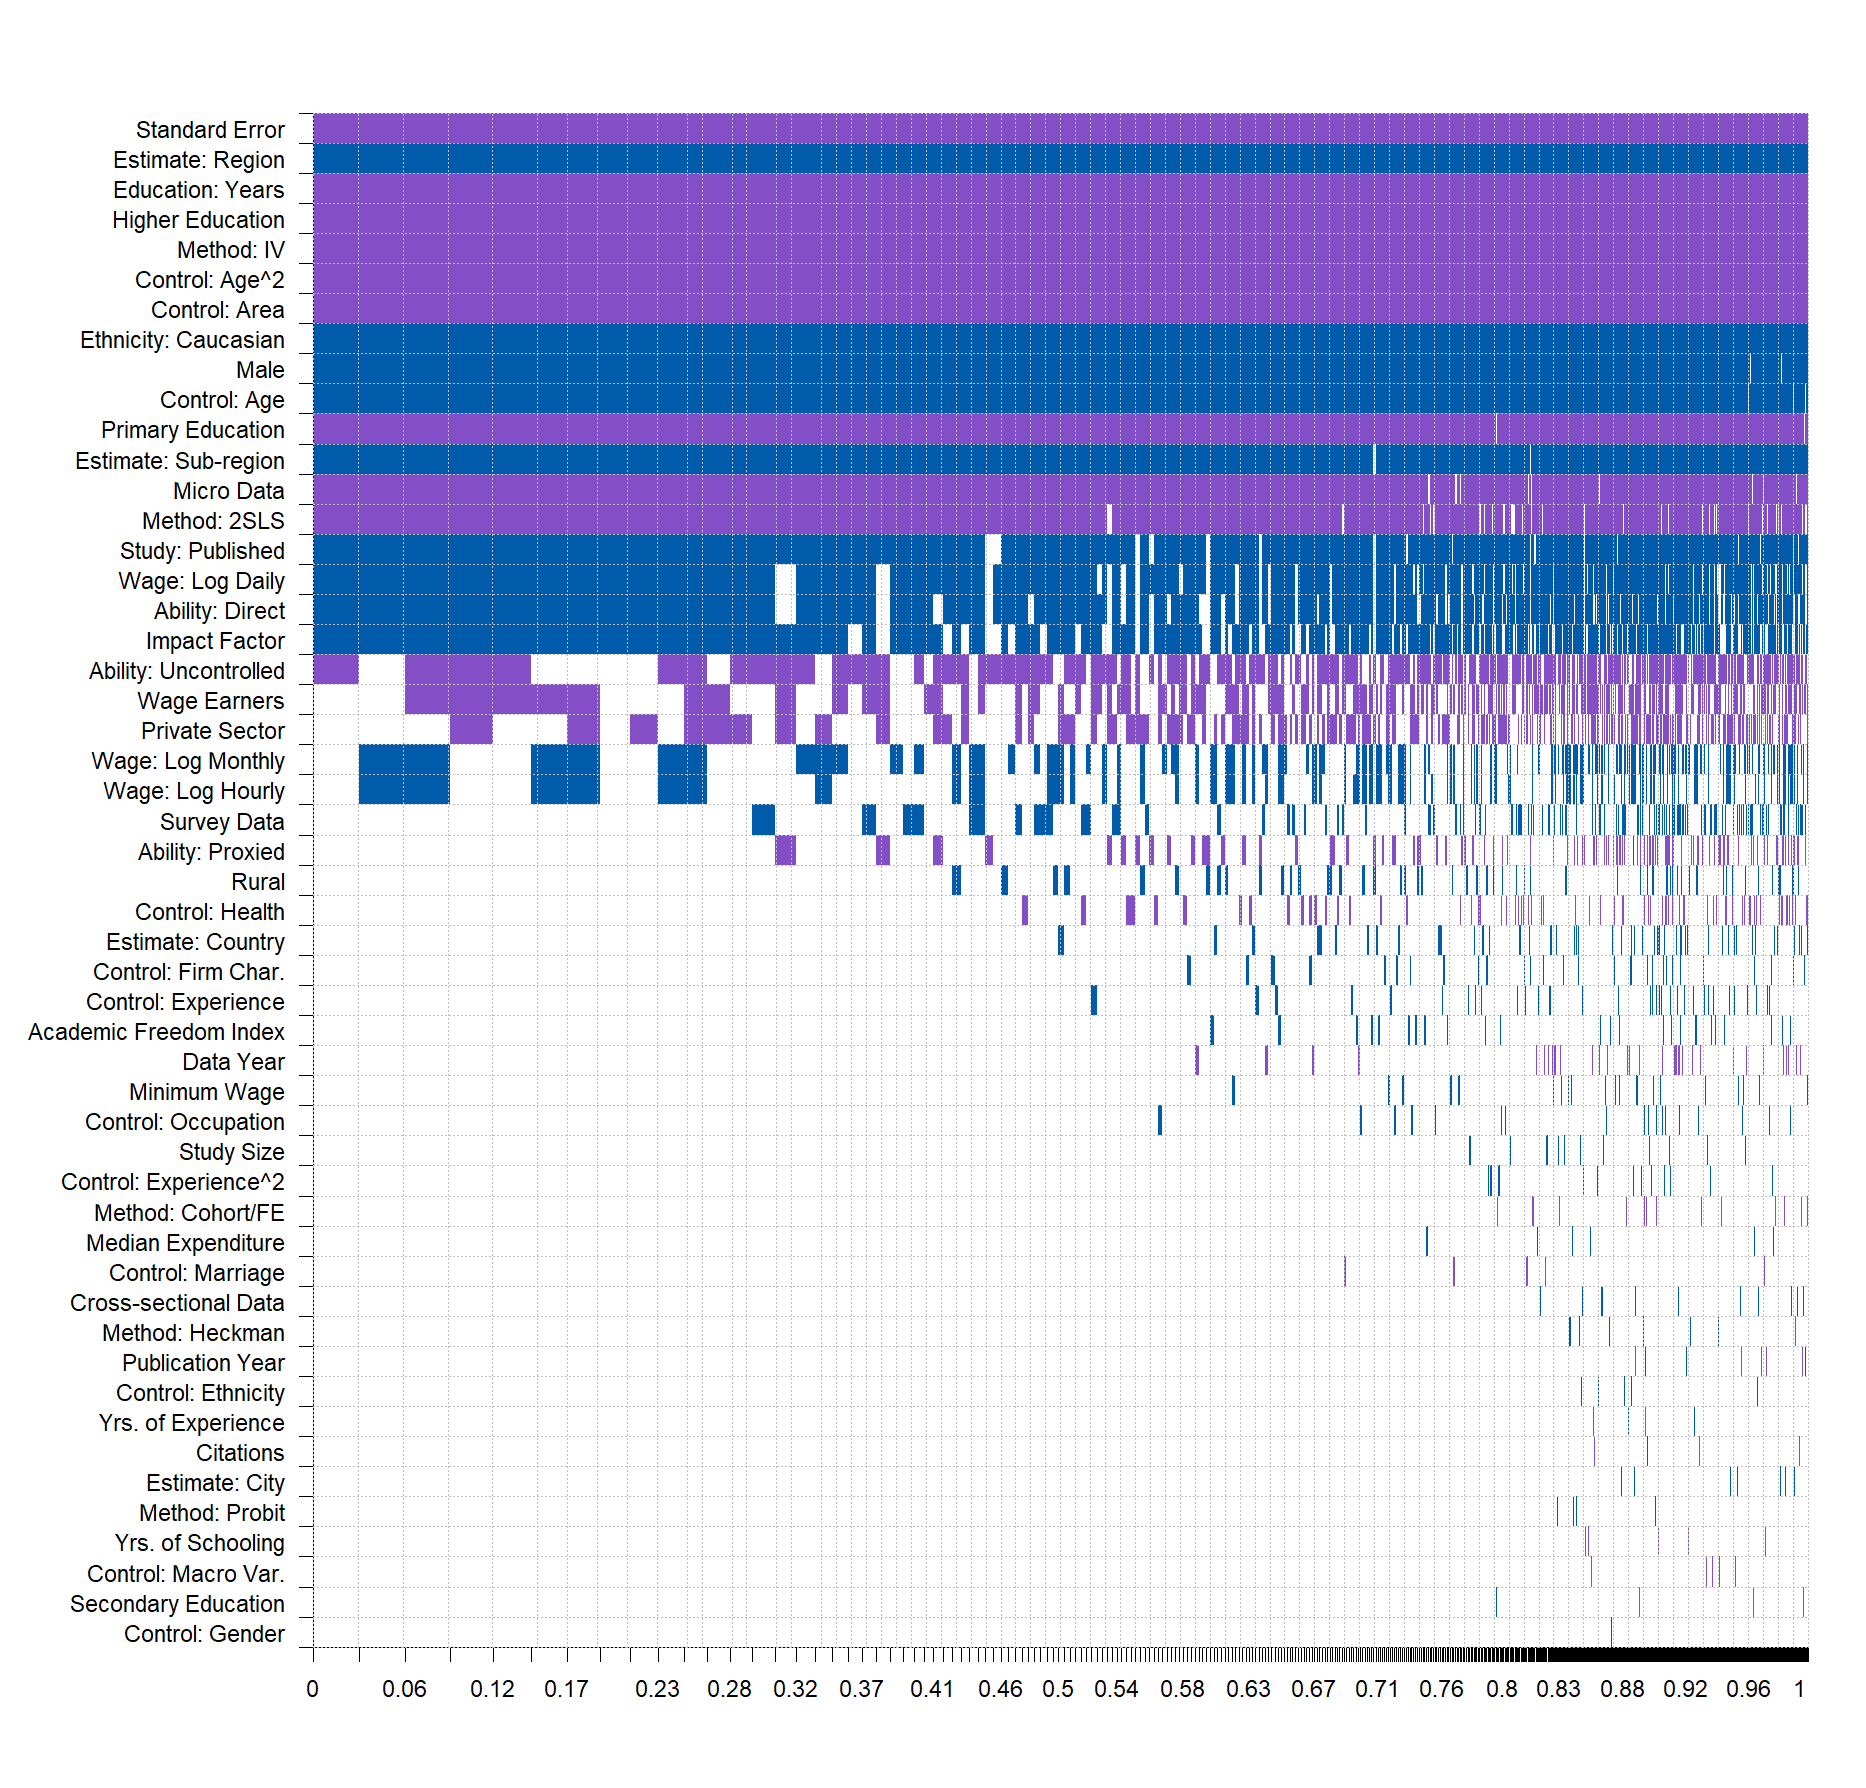
\includegraphics[width=1\textwidth]{Figures/BMA/bma_UIP_dilut_results.png}
\end{center}\vspace{-0.5cm}
\captionsetup{width=0.95\textwidth, font = scriptsize}
\caption*{\emph{Note:} This figure shows the results of the Bayesian model averaging using the uniform g-prior and dilution prior. The response variable, percentage returns to a year of schooling, is measured on the horizontal axis as cumulative posterior model probabilities. The explanatory variables are ranked in descending order on the vertical axis according to their posterior inclusion probability. Purple color (light in greyscale): the variable is included in the model and has a positive sign. Blue color (dark in greyscale): the variable is included in the model and has a negative sign. Numerical results of the estimation can be found in table \ref{tab:BMA}. For a detailed explanation of the variables, see table \ref{tab:var}.
}
\end{figure}

As an additional robustness check, I also include \ac{FMA} with Mallow's criteria for weights \citep{hansen2007least} and orthogonalization of the model space as per \cite{amini2012comparison}. The reasons for this include higher resiliency against model misspecification or the reduction of model uncertainty. In other words, \ac{FMA} provides a good sanity check that the \ac{BMA} setup is not misspecified or overly complex.

I first present graphical results in \autoref{fig:BMA}. Each variable's contribution is marked by one of two colors - purple (light in greyscale)   means a positive influence on the effect, while blue (dark in greyscale) represents a negative influence. The columns in the figure each represent a single regression model, while the rows display the inclusion of variables in these models. The left-hand side of the figure shows the best models that best fit the data. The width of each column then captures the individual model's \ac{PMP}. The proportion of models a variable is included in gives that variable's \ac{PIP}. For example, if it is included in 50\% of models, its \ac{PIP} will be 0.5. Based on the paper by \cite{kass1995bayes}, simple guidelines indicate that \ac{PIP} values between 0.5 and 0.75 suggest a weak influence on the effect, 0.75-0.9 indicate solid importance of the variable, values over 0.9 and below 0.99 mean strong influence and values over 0.99 are decisive in telling this variable is essential for explaining the effect's behavior. Even glancing into the figure, it is evident that over 15 variables have a \ac{PIP} over 0.5 in the averaging process. Looking at the fittest model, 19 variables out of 51 are included.

Next, I compare the results for both \ac{BMA} and \ac{FMA}, this time quantitatively using numeric coefficients associated with the variables. These are displayed in \autoref{tab:BMA}, where variables with \ac{PIP} over 0.5 in the \ac{BMA} have this statistic highlighted. There are 20 variables with \ac{PIP} over 0.5 in total. When it comes to \ac{FMA}, p-values of many variables are below 0.001, confirming that the models could identify a large amount of highly important effect drivers.

%BMA+FMA table
\afterpage{
\begin{singlespace}
\begin{notsotiny}
\begin{longtable}{
@{\hskip\tabcolsep\extracolsep\fill}
l
*{6}{c}
}
\caption{Model averaging results}  \label{tab:BMA}\\
\toprule
  \multicolumn{1}{l}{Response variable:} &   \multicolumn{3}{c}{Bayesian model averaging} & \multicolumn{3}{c}{Frequentist model averaging} \\
  \cmidrule(lr){2-4} \cmidrule(lr){5-7}
  \multicolumn{1}{l}{Returns to Year of Schooling} & Post. mean & Post. SD & PIP & Coef. & SE & p-value \\
\midrule
\endfirsthead
\caption[]{Model averaging results (continued)}\\
\toprule
  \multicolumn{1}{l}{Response variable:} &   \multicolumn{3}{c}{Bayesian model averaging} & \multicolumn{3}{c}{Frequentist model averaging} \\
  \cmidrule(lr){2-4} \cmidrule(lr){5-7}
  \multicolumn{1}{l}{Returns to Year of Schooling} & Post. mean & Post. SD & PIP & Coef. & SE & p-value \\
\midrule
\endhead
\bottomrule
\multicolumn{7}{r}{{\scriptsize Continued on next page}} \\
\endfoot
\endlastfoot

(Constant) & -4.729 & NaN & \textbf{1.000} & 4.838 & 350.491 & 0.989 \\
Standard Error & 0.375 & 0.064 & \textbf{1.000} & 0.516 & 0.201 & 0.010 \\
\midrule

\multicolumn{7}{l}{\emph{Estimate characteristics}}\\
Estimate: City & -0.006 & 0.081 & 0.013 & 0.000 & 1.109 & 0.000 \\
Estimate: Sub-region & -1.479 & 0.346 & \textbf{1.000} & -0.612 & 1.677 & 0.715 \\
Estimate: Region & -1.334 & 0.260 & \textbf{1.000} & -0.699 & 1.292 & 0.589 \\
Estimate: Country & -0.030 & 0.146 & 0.055 & 0.000 & 0.909 & 0.000 \\
\midrule

\multicolumn{7}{l}{\emph{Data Characteristics}}\\
Study Size & -0.002 & 0.029 & 0.014 & 0.000 & 0.373 & 0.000 \\
Yrs. of Schooling & 0.000 & 0.003 & 0.007 & 0.000 & 0.003 & 0.000 \\
Yrs. of Experience & 0.000 & 0.001 & 0.006 & 0.000 & 0.013 & 0.000 \\
Education: Years & 1.149 & 0.219 & \textbf{1.000} & 1.328 & 0.619 & 0.032 \\
Wage: Log Hourly & -0.432 & 0.465 & \textbf{0.511} & 0.000 & 0.713 & 0.000 \\
Wage: Log Daily & -1.611 & 0.623 & \textbf{0.963} & -0.595 & 1.129 & 0.598 \\
Wage: Log Monthly & -0.671 & 0.622 & \textbf{0.602} & 0.000 & 1.011 & 0.000 \\
Micro Data & 1.374 & 0.309 & \textbf{0.997} & 0.612 & 0.820 & 0.455 \\
Survey Data & -0.104 & 0.238 & 0.192 & 0.000 & 0.584 & 0.000 \\
Cross-sectional Data & -0.001 & 0.017 & 0.005 & 0.000 & 0.122 & 0.000 \\
Data Year & 1.172 & 6.961 & 0.037 & 0.000 & 46.426 & 0.000 \\
\midrule

\multicolumn{7}{l}{\emph{Spatial/structural variation}}\\
Primary Education & 3.455 & 0.855 & \textbf{0.996} & 1.409 & 2.030 & 0.488 \\
Secondary Education & -0.003 & 0.121 & 0.008 & 0.000 & 0.382 & 0.000 \\
Higher Education & 5.397 & 0.599 & \textbf{1.000} & 4.140 & 1.514 & 0.006 \\
Wage Earners & 0.882 & 0.791 & \textbf{0.621} & 0.000 & 1.411 & 0.000 \\
Male & -1.202 & 0.273 & \textbf{1.000} & -0.657 & 0.698 & 0.347 \\
Private Sector & 0.800 & 0.944 & 0.474 & 0.000 & 2.073 & 0.000 \\
Ethnicity: Caucasian & -1.460 & 0.258 & \textbf{1.000} & -1.097 & 0.546 & 0.045 \\
Rural & -0.091 & 0.338 & 0.083 & 0.000 & 1.260 & 0.000 \\
Median Expenditure & -0.004 & 0.029 & 0.032 & 0.000 & 0.164 & 0.000 \\
Minimum Wage & -0.002 & 0.020 & 0.021 & 0.000 & 0.011 & 0.000 \\
Academic Freedom Index & -0.018 & 0.126 & 0.027 & 0.000 & 0.098 & 0.000 \\
\midrule

\multicolumn{7}{l}{\emph{Estimation method}}\\
Method: Cohort/FE & 0.005 & 0.063 & 0.012 & 0.000 & 0.240 & 0.000 \\
Method: 2SLS & 1.529 & 0.411 & \textbf{0.996} & 0.640 & 0.989 & 0.517 \\
Method: Heckman & -0.001 & 0.031 & 0.006 & 0.000 & 0.063 & 0.000 \\
Method: Probit & -0.003 & 0.076 & 0.008 & 0.000 & 0.083 & 0.000 \\
Method: IV & 2.651 & 0.348 & \textbf{1.000} & 1.701 & 0.901 & 0.059 \\
Ability: Direct & -1.218 & 0.486 & \textbf{0.930} & -0.632 & 0.699 & 0.366 \\
Ability: Proxied & 0.085 & 0.277 & 0.104 & 0.000 & 0.924 & 0.000 \\
Ability: Uncontrolled & 0.492 & 0.406 & \textbf{0.696} & 0.000 & 0.950 & 0.000 \\
Control: Age & -1.921 & 0.408 & \textbf{1.000} & -0.983 & 1.106 & 0.374 \\
Control: Age$^2$ & 2.992 & 0.432 & \textbf{1.000} & 2.049 & 1.118 & 0.067 \\
Control: Experience & -0.021 & 0.118 & 0.042 & 0.000 & 0.686 & 0.000 \\
Control: Experience$^2$ & -0.001 & 0.025 & 0.007 & 0.000 & 0.185 & 0.000 \\
Control: Ethnicity & 0.000 & 0.022 & 0.006 & 0.000 & 0.206 & 0.000 \\
Control: Health & 0.049 & 0.188 & 0.080 & 0.000 & 0.600 & 0.000 \\
Control: Gender & 0.000 & 0.011 & 0.002 & 0.000 & 0.241 & 0.000 \\
Control: Marriage & 0.003 & 0.038 & 0.015 & 0.000 & 0.254 & 0.000 \\
Control: Occupation & -0.009 & 0.079 & 0.019 & 0.000 & 0.005 & 0.000 \\
Control: Firm Char. & -0.022 & 0.121 & 0.045 & 0.000 & 0.597 & 0.000 \\
Control: Area & 1.784 & 0.234 & \textbf{1.000} & 0.840 & 1.083 & 0.438 \\
Control: Macro Var. & 0.000 & 0.019 & 0.007 & 0.000 & 0.126 & 0.000 \\
\midrule

\multicolumn{7}{l}{\emph{Publication characteristics}}\\
Impact Factor & -0.215 & 0.088 & \textbf{0.931} & -0.105 & 0.165 & 0.524 \\
Citations & 0.000 & 0.006 & 0.006 & 0.000 & 0.111 & 0.000 \\
Study: Published & -1.157 & 0.280 & \textbf{0.999} & -0.430 & 1.242 & 0.730 \\
Publication Year & 0.000 & 0.017 & 0.003 & 0.000 & 0.044 & 0.000 \\
\bottomrule
\addlinespace[0.2em]

\multicolumn{7}{>{\scriptsize}p{0.95\linewidth}}{\emph{Note:} This table presents the results of the Bayesian and Frequentist model averaging. Post. mean = Posterior Mean, Post. SD = Posterior Standard Deviation, PIP = Posterior Inclusion Probability, Coef. = Coefficient, SE = Standard Error, OLS = Ordinary Least Squares, FE = Fixed Effects, 2SLS = 2 Stage Least Squares. The variables with PIP > 0.5 are highlighted. For a detailed explanation of the variables, see table \ref{tab:var}.}
\end{longtable}
\end{notsotiny}
\end{singlespace}
\clearpage
}

Looking at these in more detail, the publication bias stands out immediately. Despite the mixed or otherwise lukewarm claims about its presence in \autoref{chap:four}, both presented models strongly suggest that publication bias appears in the data. The standard error coefficients are 0.375 and 0.516 for both respective models; both these coefficients are statistically significant. The \ac{PIP} of 1.000 associated with the coefficient in the \ac{BMA} model is the highest possible, and the p-value for the \ac{FMA} model is also below 0.01.

Let us now explore those variables that negatively influence the effect. Firstly, regional and sub-regional data appear to diminish the effect's magnitude, as does reporting the wage in daily units or having a male or Caucasian subject group. Furthermore, published studies are likewise associated with lower effect in both models, although the \ac{FMA} p-value tied to this claim does not hold enough significance. While the linear age coefficient pulls the effect heavily in the negative direction, the quadratic coefficient works in the opposite direction, ultimately contributing positively to the overall effect. Perhaps the most interesting out of the negative drivers, however, is the direct ability variable. Out of the other ability variables, it is associated with the highest \ac{PIP} and has the biggest influence on the effect. This potential evidence for ability bias is weakened only by the \ac{FMA} robustness check, where the p-value is not small enough to claim statistical significance.


Regarding variables that exert a positive influence on the effect as opposed to a negative one, two coefficients stand out the most. These are, first, primary education; second, higher education. Although the secondary education coefficient is insignificant for the \ac{BMA} model, this may further prove that education truly matters. Apart from this foreseeable conclusion, we can also see that data collected on the micro level positively influence the overall effect, as does estimating the equation using 2-stage least squares or an instrumental variable regression. Controlling for the type of area in which the subjects work also has a significant positive effect, as do the earlier mentioned age squared and standard error. Lastly, I would like to give attention to the \textit{Education: Years} variable, which also exhibits a significant positive impact on the effect. In line with \cite{churchill2018meta}, reporting the estimates in years rather than levels seems to be of systematic importance rather than a fluke. I can think of two sources of this phenomenon - the functional form of \autoref{eq:schooling_levels} and human error. While the former may be induced purely by imperfect modeling of the relationship between an attained level of education and the returns associated with each year spent studying for that level, the latter appears less streamlined. Given that all estimates reported in levels had to be transformed and unified using a calculation with incomplete information (sometimes the number of years necessary to finish a certain degree was missing), this uncertainty may give rise to the systematic influence we observe.

As the last piece of information added to the model averaging topic, I also present the differences between posterior inclusion probabilities of models ran under different specifications, namely different priors. Apart from the above-mentioned uniform g-prior and dilution model prior, I run the estimation for three unique pairs of priors. These are, listed in an arbitrary order, uniform g-prior \& uniform model prior, benchmark g-prior \& random model prior, and Hannah-Quin criterion g-prior \& random model prior. The posterior inclusion probabilities of variables ran under all these specifications are displayed in \autoref{fig:BMA_comparison}. The results appear highly stable and invariable towards different specifications, and I find no further need to dig deeper in this regard. For a graphical display of results under each of the three additional specifications, see \autoref{app:three}.

\begin{figure}[!t]
\begin{center}
\caption{Inclusion probability varies little across different model specifications}
\label{fig:BMA_comparison}
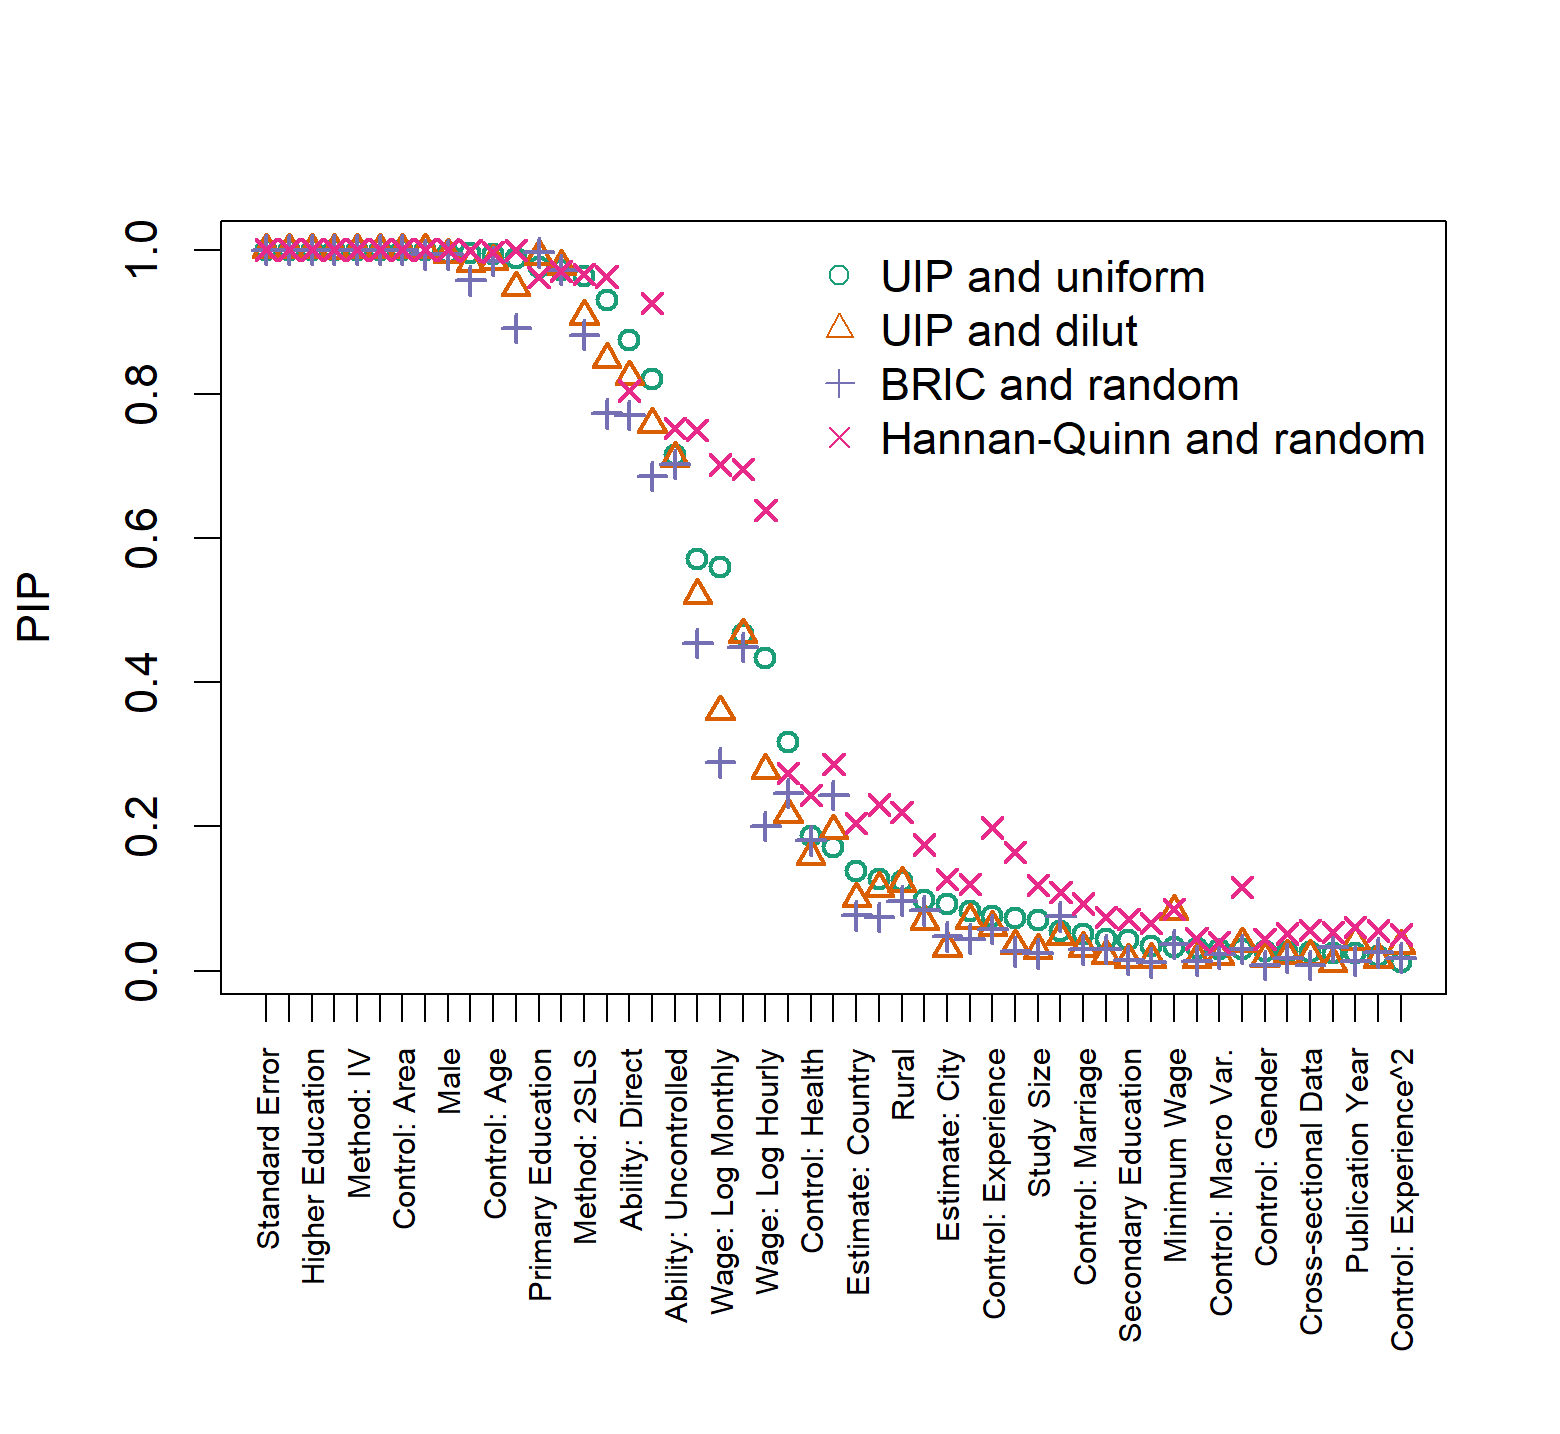
\includegraphics[width=0.8\textwidth]{Figures/BMA/bma_comparison.png}
\end{center}\vspace{-0.5cm}
\captionsetup{width=0.8\textwidth, font = scriptsize}
\caption*{\emph{Note:} This figure shows how much variables used in Bayesian model averaging contribute to the returns to education effect under different model specifications. The variables are displayed on the x-axis against their posterior inclusion probabilities on the y-axis. PIP = Posterior Inclusion Probability, UIP = Uniform g-prior, Dilut = Dilution Prior, Uniform = Uniform Model Prior, BRIC = Benchmark g-prior, Random = Random Model Prior, HQ = Hannan-Quinn Criterion. For the explanation of the variables and their detailed interpretation, see table \ref{tab:var}.}
\end{figure}

This concludes the chapter on model averaging. In \autoref{app:three}, you may find several robustness check figures, including the correlation table of utilized variables, graphical results, and a comparison of \ac{BMA} models ran under different specifications.

